\section{RESULTS}
\subsection{CO EMISSIONS AND LINE RATIOS}

\begin{figure*}[htbp]
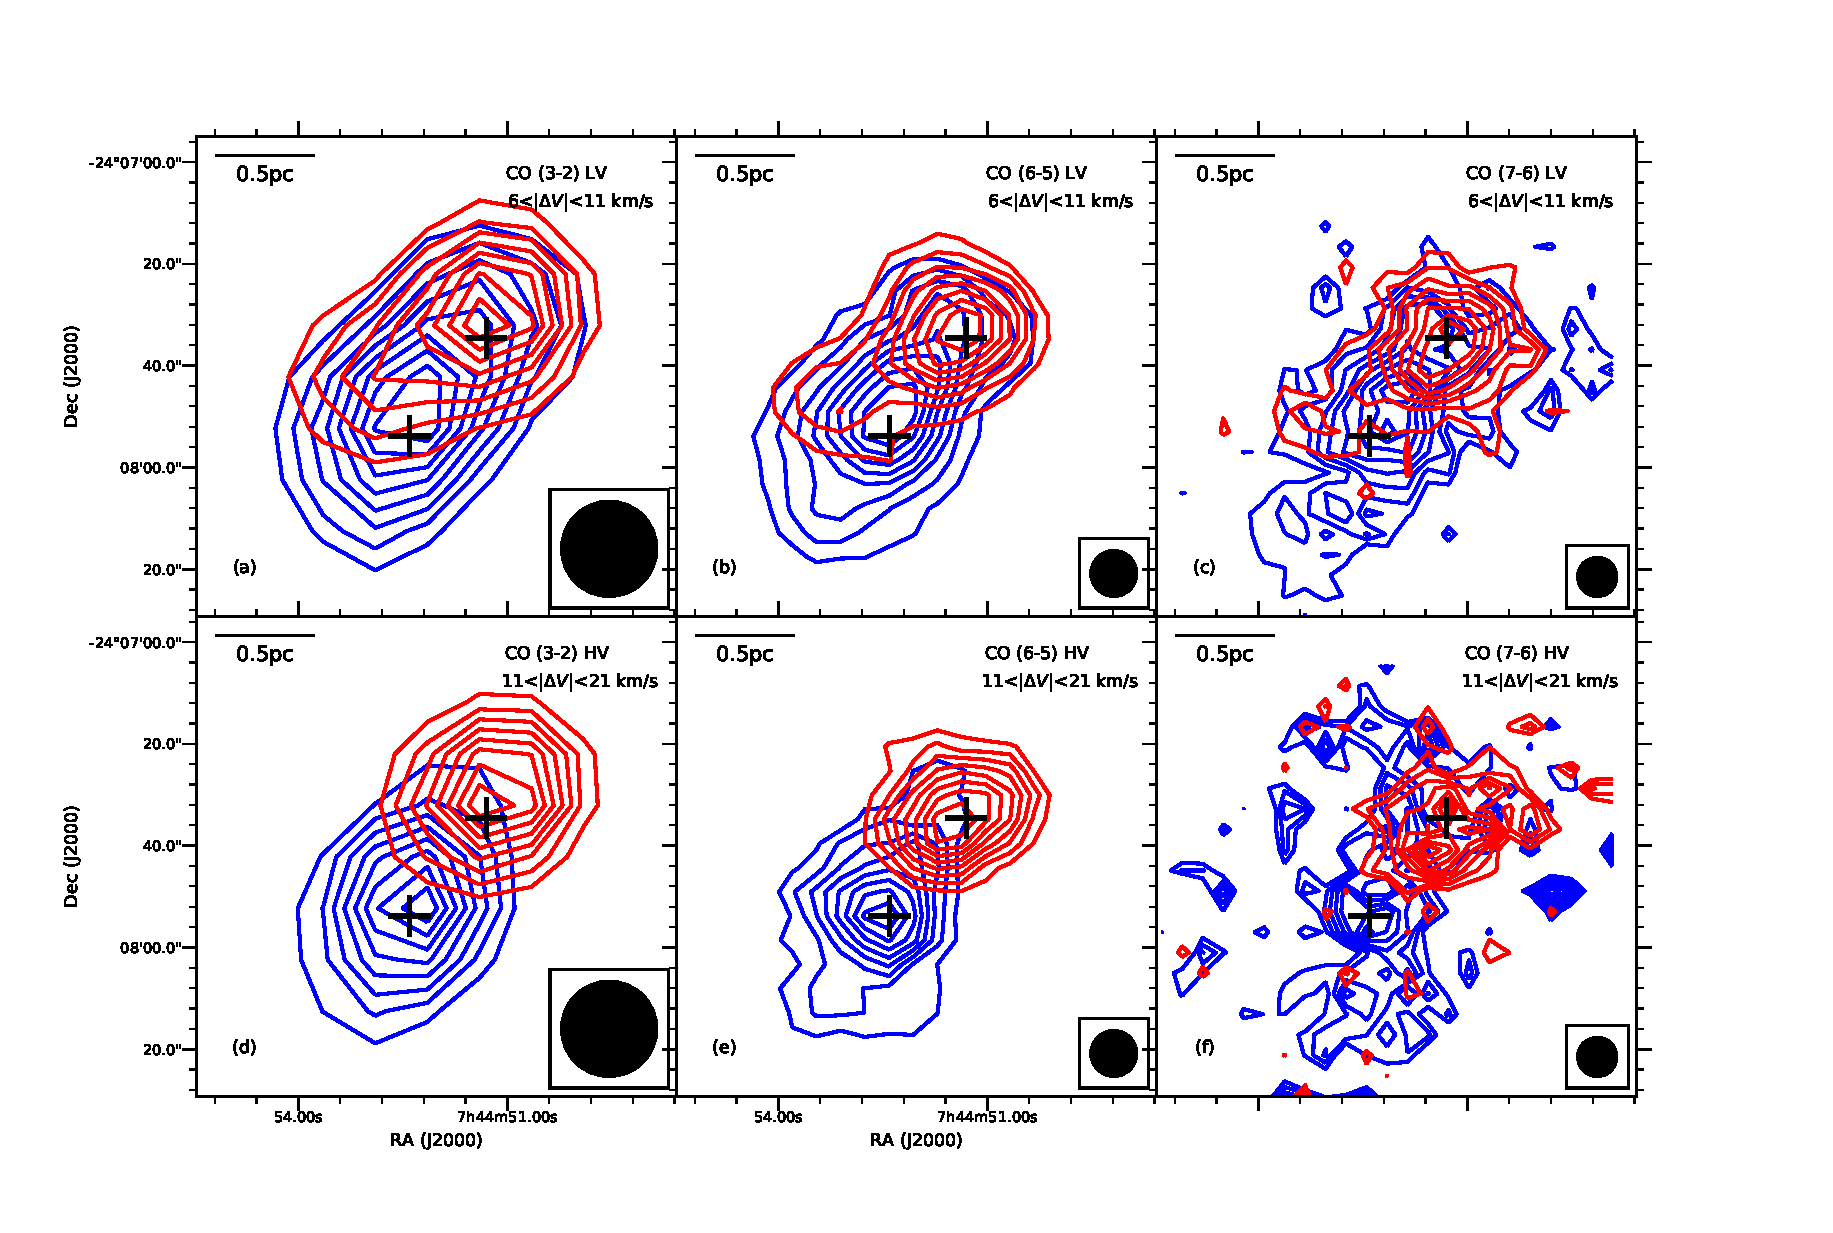
\includegraphics[scale=.60]{./fig/ori_contour.eps}
\caption{(a)-(c) Low-velocity CO J = (3-2), (6-5), (7-6) emissions, integrated from $-11$ to $-6$ (blue) and $6$ to $11$ (red) km s$^{-1}$ ; (d)-(f) High-velocity CO J = (3-2), (6-5), (7-6) emissions,  integrated from $-21$ to $-11$ (blue) and $11$ to $21$ (red) km s$^{-1}$. All velocities are with respect to the v$_{\mathrm{cloud}}$. For (a)-(f), the contour levels start from 20\% and continue at steps of 10\% of the peak emission. The central stars mark the positions of the millimeter sources detected by \citet{2009ApJ...696...66Q}. The beam size is shown in the lower right corner of each panel.  \label{fig1}}
\end{figure*}

The cloud velocity (v$_{\mathrm{cloud}}$) with respect to the local standard of rest is about 67.5 km s$^{-1}$, which is adopted from \citet{2003A&A...412..175K}. Figure \ref{fig1} shows the integrated low-velocity (LV) and high-velocity (HV) emissions of CO J = (3-2), (6-5), (7-6). The outflow morphologies seen in three lines are very similar. For all transitions, a prominent bipolar outflow at (PA) $\sim$ 131${\degr}$ along with a weaker component at PA $\sim$ 101${\degr}$ is detected. The weaker component is at relatively lower velocities of $\pm$6 to $\pm$11 km s$^{-1}$, while the prominent component is detected at both low and high velocities. The signal-to-noise ratio in the CO (7-6) spectrum is not very high at high velocities. Overall, the CO maps presented in Figure \ref{fig1} are very similar to the CO (3-2) map presented by \citet{2003A&A...412..175K}. 

To compare the emissions of different CO transitions, we convolved the CO (6-5) and (7-6) maps, as well as the CO (2-1) map from \citet{2009ApJ...696...66Q}, to the same spatial resolution of the CO (3-2), which is 19${\arcsec}$. To reduce the noise level in the spectra, we resampled the four CO lines to a resolution of 2 km s$^{-1}$. Then we measured ratios of the main beam temperature ($T_{\mathrm{mb}}$) of different CO lines toward the peak of the blueshifted and redshifted lobes (marked as two crosses in each panel of  in Figure \ref{fig1}). Figure \ref{fig2} shows the observed line wing ratios of different CO transitions.  All line ratios in Figure \ref{fig2} are remarkably constant with velocity.

\begin{figure}[tbp]
\plotone{./fig/ratio.eps}
\caption{Ratios of the $T_{\mathrm{mb}}$ of different CO lines at various velocities. Blue symbols denote the measurements from the blueshifted lobe, and red symbols the redshifted lobe. The $V_{\mathrm{outflow}}$ shown here is related to the $v_{\mathrm{cloud}}$ by the relation: $V_{\mathrm{outflow}}$ = $\mid$ $v_{\mathrm{outflow}}$ - $v_{\mathrm{cloud}}\mid$, where $v_{\mathrm{outflow}}$ is the outflow velocity with respect to the local standard of rest. \label{fig2}}
\end{figure}

\subsection{PHYSICAL PROPERTY ANALYSIS}
We measure the main beam temperature ($T_{\mathrm{mb}}$) of four CO lines at the peak position of the blue lobe and the red lobe (marked as two crosses in each panel of Figure \ref{fig1}). Because the $^{13}$CO emission is not detected in the outflowing gas, the four transitions of $^{12}$CO are assumed to be optically thin during our analysis. Using the RADEX code \citep{2007A&A...468..627V}, we construct a large grid of non-LTE models with three parameters: gas density ($n_{\mathrm{H}_2}$), kinetic temperature ($T_{\mathrm{kin}}$), and CO column density ($N_{\mathrm{CO}}$). Linewidths are given as input and are fixed to 2 km s$^{-1}$. The physical parameters in the outflow can be derived by comparing the main beam temperatures of various transitions with the model line intensities. Because of the degeneracies of the source size with the CO column density (in the optically thin case), all the computations are done assuming that the beam-filling factor is one for each transition. Thus, the derived physical parameters of the gas are beam-averaged values. 

The best fit is obtained by minimizing the reduced $\chi^2$ ($\chi^2_{\mathrm{red}}$) between the observed data and the model intensities using the Levenberg-Marquardt method \citep{1992nrfa.book.....P}. With four line observations and three simulation parameters, our fitting has one degree of freedom. At velocities where the CO (7-6) emission is not detected, the best fit is obtained by minimizing $\chi^2$ instead of $\chi^2_{\mathrm{red}}$. During the fitting, the intensity uncertainties of CO (2-1), CO (3-2), CO (6-5), CO (7-6) are set to 0.15, 0.2, 0.25, 0.3 respectively.  We find that values of the $\chi^2_{\mathrm{red}}$ of the best fitting results at most velocities are much less than 1, indicating that we might be a bit conservative at the intensity uncertainty or the real value of degrees of freedom is smaller than one \citep{2010arXiv1012.3754A}. To get more reasonable uncertainties of each fitted parameter, we divide the $\chi^2_{\mathrm{red}}$ by an appropriate factor to make $\chi^2_{\mathrm{red}}$ approach 1 at most velocities. However, the $\chi_{\mathrm{red}}^2$ at some velocities remains much less than 1 after the division procedure. As show in Figure \ref{fig5a}, the upper limits of gas temperatures would be anomaly high at these velocities. 

\begin{figure}[tbp]
\centering
\subfigure[]{
\begin{minipage}[b]{0.5\textwidth}
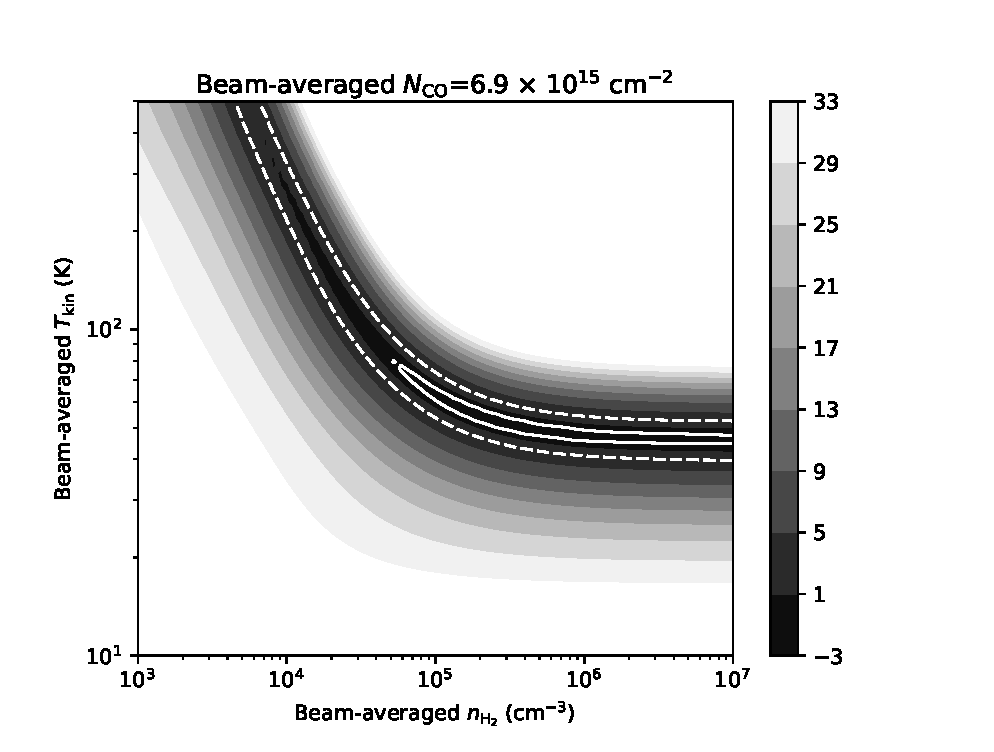
\includegraphics[width=1\textwidth]{./fig/chiimage_nco_paper.eps}
\label{fig3a}
\end{minipage}
}
\subfigure[]{
\begin{minipage}[b]{0.5\textwidth}
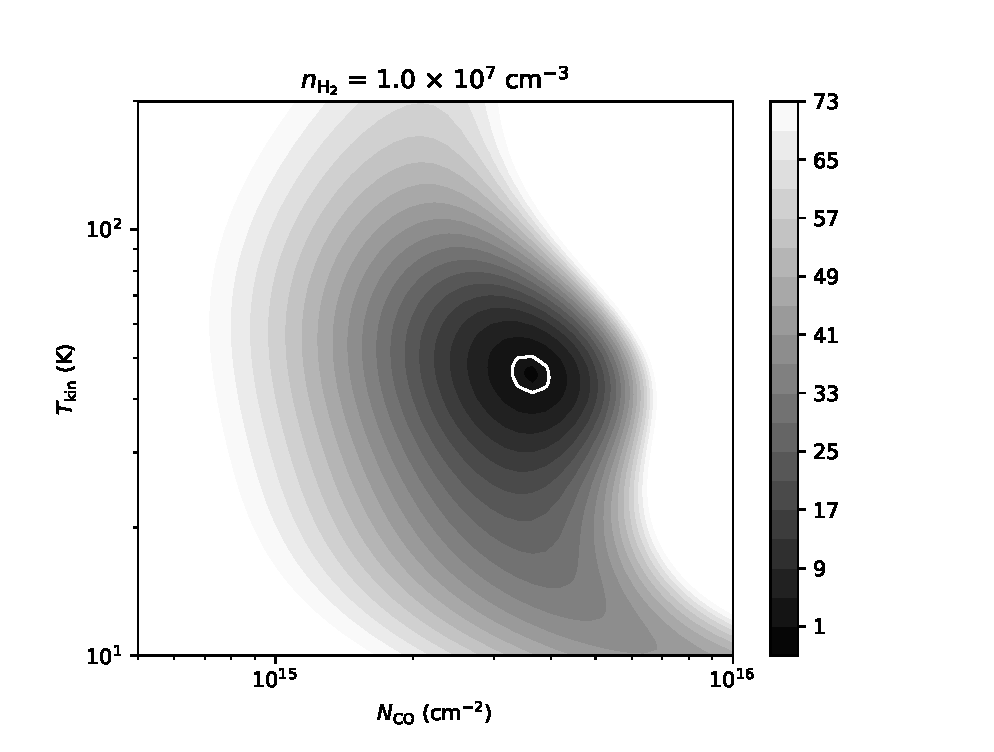
\includegraphics[width=1\textwidth]{./fig/chiimage_nh2_paper.eps}
\label{fig3b}
\end{minipage}
}
\subfigure[]{
\begin{minipage}[b]{0.5\textwidth}
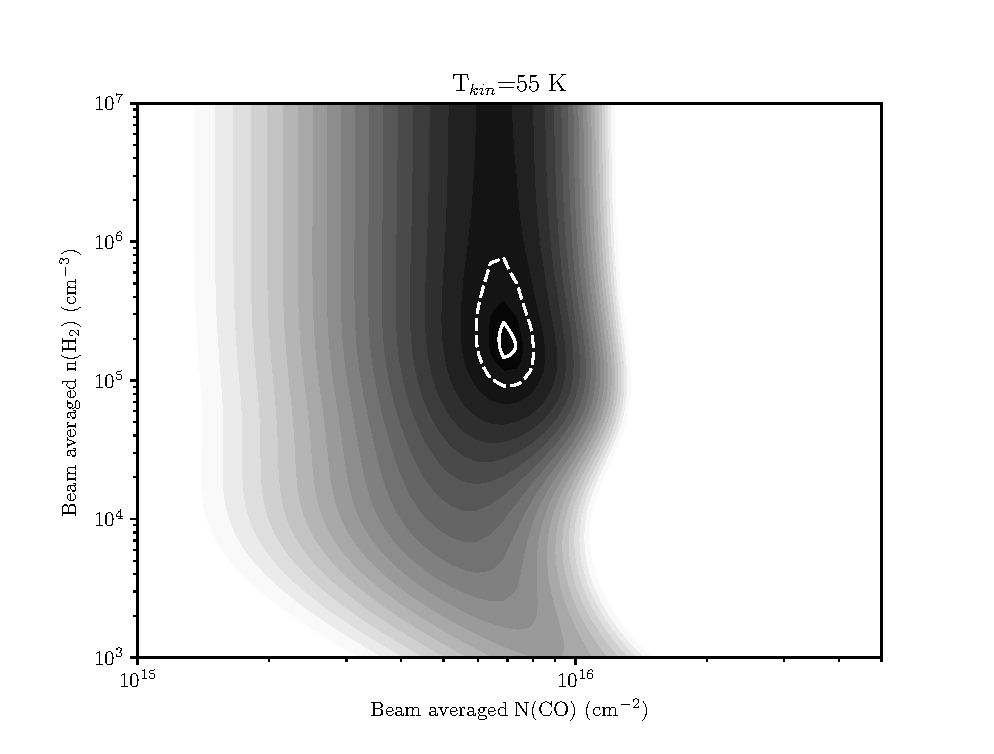
\includegraphics[width=1\textwidth]{./fig/chiimage_tkin_paper.eps}
\label{fig3c}
\end{minipage}
}
\caption{The $\chi_{\mathrm{red}}^2$ distribution for G240 outflow at 58 km s$^{-1}$ in the (a) [$T$, $n$], (b) [$T$, $N$], (c) [$n$, $N$] planes, with all other parameters fixed to the parameters of the best fitting results at this velocity. Solid contours and dashed contours show the 1$\sigma$ and 3$\sigma$ confidence levels respectively. \label{fig3}}
\end{figure}

In Figure \ref{fig3}, we show cuts in the $\chi_{\mathrm{red}}^2$ along the [$T$, $n$], [$T$, $N$], [$n$, $N$] planes at 58 km s$^{-1}$ as examples of the $\chi_{\mathrm{red}}^2$ distribution, with all the other parameters fixed to the parameters of the best fitting result at this velocity. As shown in Figure \ref{fig3b} and Figure \ref{fig3c}, the $\chi_{\mathrm{red}}^2$ has only one minimum in [$T$, $n$], [$T$, $N$] planes. However, Figure \ref{fig3a} shows that the gas is thermalized and no upper limits to the density could be derived. The $\chi_{\mathrm{red}}^2$ distribution behaves similarly at other velocities. 

We compare the LVG results with a population diagram analysis under the local thermal equilibrium assumption \citep{1999ApJ...517..209G}. Throughout the population diagram analysis, we assume that the outflow emission is optically thin. The population of each level is given by 
\begin{equation}
N_{\mathrm{up}} = \frac{N_\mathrm{CO}}{Z} g_\mathrm{up} e^{-E_\mathrm{up}/kT_\mathrm{kin}},
\end{equation}
where $N_\mathrm{up}$ is the column density in the upper state, $g_\mathrm{up}$ the statistical weight of the upper state, $E_\mathrm{up}$ the upper energy level, $k$ the Boltzmann constant, and Z is the partition function.
Population diagram for CO at 58 km s$^{-1}$ as an example is shown in Figure \ref{fig4}. The molecular energy levels are in Boltzmann distribution. The population diagram behaves similarly at other velocities. Figure \ref{fig5} shows the outflowing gas temperature and the CO column density, estimated from the LVG analysiss and the population diagram analysis, as functions of gas velocity. The $N$-$V$ diagram shows a clear decreasing trend of CO column density with outflow velocity, while the $T$-$V$ diagram shows that the gas temperature has no obvious dependence on gas velocity. At velocities where we have more lines than parameters to fit, we derive the uncertainties of each parameter of the LVG analysis from the 1$\sigma$ confidence region in the $N$-$T$-$n$ 3-dimensional space. The 1$\sigma$ temperature uncertainties of the LVG analysis are shown in Figure \ref{fig5a}. The lower limits of gas density ($n_{\mathrm{lower}}$) are around 10$^5$ cm$^{-3}$ at most velocities. At velocities where $\chi_{\mathrm{red}}^2 \ll 1$, $n_{\mathrm{lower}}$ could be as low as $3 \times 10^4$ cm$^{-3}$. The uncertainties of the CO column densitiy are $\sim$ 10 \%. 

\begin{figure}[tbp]
\plotone{./fig/rotationT58.eps}
\caption{Population diagram for CO at 58 km s$^{-1}$.  The fitted line shows the Boltzmann distribution of the rotational populations. \label{fig4}}
\end{figure}

\begin{figure}[htbp]
\centering
\subfigure[]{
\begin{minipage}[b]{0.5\textwidth}
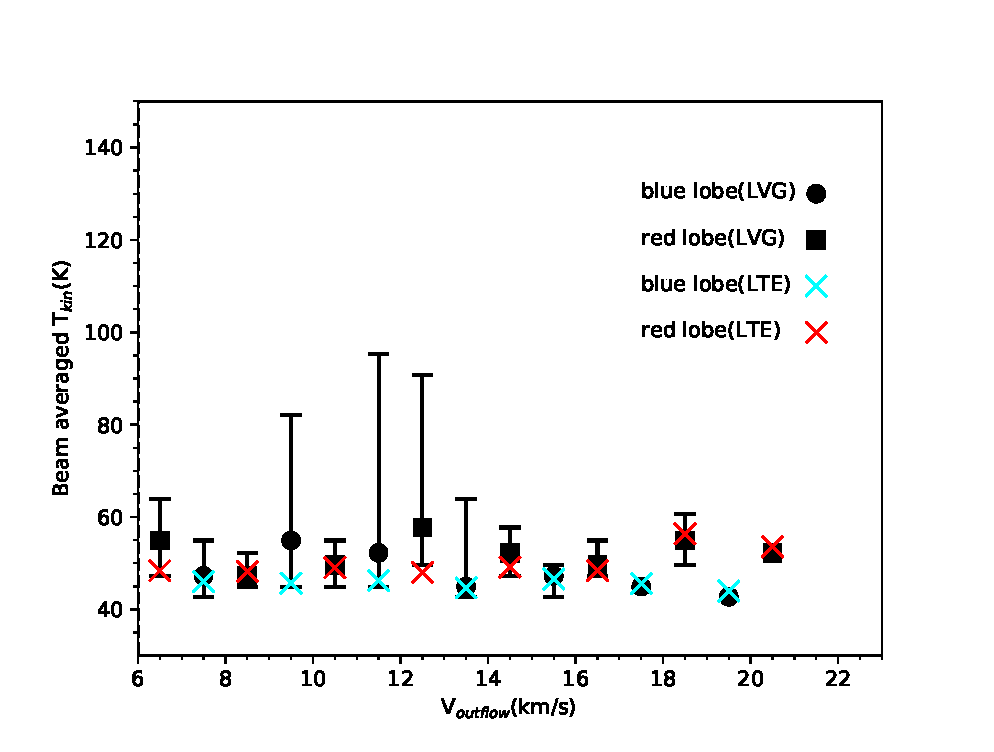
\includegraphics[width=1\textwidth]{./fig/tv_paper.eps}
\label{fig5a}
\end{minipage}
}
\subfigure[]{
\begin{minipage}[b]{0.5\textwidth}
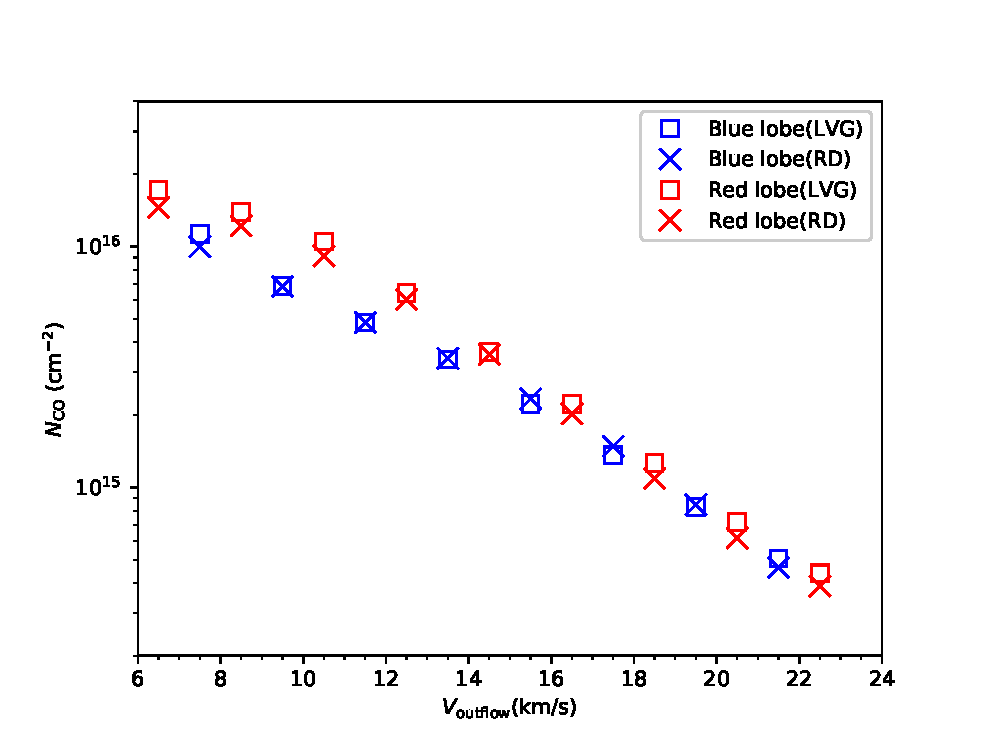
\includegraphics[width=1\textwidth]{./fig/Nv_paper.eps}
\label{fig5b}
\end{minipage}
}
\caption{$T$-$V$ and $N$-$V$ diagrams of the G240 outflow, estimated from LVG analysis (black open circles for blue lobe and black open squares for red lobe) and population diagram analysis (blue x marker for blue lobe and red x marker for red lobe). The 1$\sigma$ temperature uncertainty estimated from the LVG analysis is shown in the $T$-$V$ diagram (error bars). \label{fig5}}
\end{figure}


